
\chapter{Evaluation}

As stated in previous chapters, the Learning Analytics Software was created with two main objectives. The first is to monitor the performance of the students in different levels: individual, per quiz and per group. The second is to ease the understanding of the items in online quizzes to improve the design of future quiz items \footnote{so that the instructor could quickly adapt the quizzes to the needs of the students in the group}. These two objectives were evaluated with a focus group that consisted of 3 persons working with online quizzes and interested in learning analytics topics. 

\section{Focus group structure}

The general structure of the focus group consists of two big sections of 30 minutes each. The first was a general introduction to the Learning Analytics objectives, the implemented models, and its capabilities. During this section, a sheet of paper with a series of questions related to objective accomplishment was provided. The next 30 minutes of the focus group consisted of a user interface evaluation, where a synthetic dataset and a series of tasks where given, then the participants had to evaluate some affirmations about the usability.

\subsection{Participants}
For the focus group, eleven persons were invited via email to participate in this focus group. All of them are faculty members of the University of Edinburgh and had shown an interest in online learning tools. Due to their busy agenda, only three of them could assist. All of them professors from the School of Medicine. This focus group was conducted by a moderator.

\subsection{Synthetic dataset}

To test the usability of the first version of the lanalytics package and dashboard, a synthetic dataset was created. This dataset consists of 12 quiz data files, one file for the cognitive levels and one file containing the final grades of the students. These were specially designed to show some specific patterns in the plots, so in this section, the dataset will be described. 

To generate the 100 email users a 10-character string was randomly generated, then each of these students was assigned to one of three groups (thinking of subpopulations inside the same group; for example, students that usually get high scores, students that get medium scores and students that get low scores). Then, for each email, 12 quizzes with 11 question each were generated. 

Now, the probability of obtaining the right answer for each question was distributed as a Bernoulli distribution with distinct probability according to the group that the user belongs (of the three groups randomly generated). The \cref{tbl:probabilities} states the exact probabilities for each subpopulation and item.

\begin{table}[ht!]
\centering
\caption{Probability to get correct the answer}
\label{tbl:probabilities}
\begin{tabular}{|l|l|l|l|}
\hline
Item & \begin{tabular}[c]{@{}l@{}}High skilled\\ students\end{tabular} & \begin{tabular}[c]{@{}l@{}}Medium skilled\\ students\end{tabular} & \begin{tabular}[c]{@{}l@{}}Low skilled\\ students\end{tabular} \\ \hline
1    & 0.83                                                            & 0.73                                                              & 0.63                                                           \\ \hline
2    & 0.85                                                            & 0.75                                                              & 0.65                                                           \\ \hline
3    & 0.90                                                            & 0.80                                                              & 0.70                                                           \\ \hline
4    & 0.95                                                            & 0.85                                                              & 0.75                                                           \\ \hline
5    & 0.95                                                            & 0.90                                                              & 0.80                                                           \\ \hline
6    & 0.70                                                            & 0.65                                                              & 0.60                                                           \\ \hline
7    & 0.70                                                            & 0.65                                                              & 0.60                                                           \\ \hline
8    & 0.95                                                            & 0.85                                                              & 0.75                                                           \\ \hline
9    & 0.85                                                            & 0.80                                                              & 0.70                                                           \\ \hline
10   & 0.85                                                            & 0.85                                                              & 0.85                                                           \\ \hline
11   & 0.70                                                            & 0.60                                                              & 0.50                                                           \\ \hline
\end{tabular}
\end{table}

Now, for the answering time per question, two assumptions were taken. The first is that the date for any answer of quiz one might be answered before of the date of any question of quiz 2 and so on. To ensure this, each quiz was in differents months. Now, for the answering time of the questions in the same quiz, it was assumed that the students answered the quiz in order and in a continuous consecutive interval of time. Then, if we calculate the time difference between the two questions, it would represent the spent time in the question. To create this synthetic variable,  a normal distribution with different mean and standard deviation was used.

The final exam file was generated with the same users as the quizzes files, and the final grade was normally distributed with a centre in the student mean score of the quizzes. Finally, the cognitive file was generated based on the probabilities of getting correct a question \cref{tbl:probabilities}. This way, the items that were easier would have a cognitive level of 1 (the easiest one) and consecutively until the cognitive level 3. 


\section{Focus group}

\subsection{Introduction of the software (30 minutes)}

This section of the focus group is divided into two parts, one of 10 minutes and the other of 20 minutes. The first part is to introduce the capabilities of R and Shiny to motivate future uses and further implementations. The second part is an introduction of the Learning Analytics Package objectives and its Shiny interface. In this phase, the motivation of the models and the generated plots were explained.

As part of the evaluation, five questions were asked in a sheet of paper for each of the participants. The objective was to discuss if the presented models were consistent with the objectives. The list of the five questions presented are the following:
  
  \begin{itemize}
\item{Do the shown figures in the \textbf{Individual analysis} help you to monitor how an individual student is performing? What else would you like to understand about the student?}
\item{Do the shown figures in the \textbf{Group analysis} help you to monitor how the group is performing?  What else would you like to understand about the group?}
\item{Do the shown figures in the \textbf{Quiz analysis} help you to understand the difficulty of the items as well as the required time per quiz? What are the main points that you consider when designing an item of a quiz?}
\item{The \textbf{Rasch model} helps you to understand the easiness-difficulty of your items?}
\item{The Rasch model plots \textbf{(ICC, Person-Item, Person-parameter)} gave you actionable information to improve the design of your quizzes?}
\end{itemize}

\subsection{User experience evaluation (30 minutes)}

Once the presentation of the software is concluded, the synthetic dataset is provided and a 20 minutes user experience evaluation starts. In this part, the users have ten tasks to accomplish [\cref{tbl:tasks}], with the central objective to evaluate the usability of the dashboard. In particular, they have to evaluate the easiness of the instructions as well as the easiness of the elements in the dashboard.

\begin{table}[ht!]
\centering
\caption{Tasks to accomplish}
\label{tbl:tasks}
\begin{tabular}{|l|l|}
\hline
\textbf{Tab}            & \textbf{Task}                                                                                                                     \\ \hline
Import quizzes tab      & Upload the quizzes files                                                                                                          \\ \hline
Import quizzes tab      & \begin{tabular}[c]{@{}l@{}}Upload the cognitive file and the final \\ exam file\end{tabular}                                      \\ \hline
Import quizzes tab      & Remove the cognitive file and upload it again                                                                                     \\ \hline
Display quizzes tab     & View if the uploaded files are correct                                                                                            \\ \hline
Display quizzes tab     & \begin{tabular}[c]{@{}l@{}}Select the Item and the Cognitive level column \\ for the cognitive file.\end{tabular}                 \\ \hline
Individual Analysis tab & Search one student and view its grades.                                                                                           \\ \hline
Group Analysis tab      & \begin{tabular}[c]{@{}l@{}}Select one quiz and view the guessers and \\ order plot\end{tabular}                                   \\ \hline
Quiz Analysis tab       & Observe the histogram and boxplot.                                                                                                \\ \hline
Quiz Analysis tab       & \begin{tabular}[c]{@{}l@{}}Observe the ET and ETL plot. Do you see \\ some pattern with the cognitive level?\end{tabular}         \\ \hline
eRm package tab         & \begin{tabular}[c]{@{}l@{}}Select one file and view the ICC, the person \\ item map and the person, parameters plot.\end{tabular} \\ \hline
\end{tabular}
\end{table}

To measure the usability of the dashboard, some affirmations are given, and the users have to agree with them according to a Likert scale (1 = Strongly disagree, 2 = Disagree, 3 = Neutral, 4 = Agree, 5 = Strongly agree) [\cref{tbl:likert1}].

\begin{table}[ht!]
\centering
\caption{Likert evaluations}
\label{tbl:likert1}
\begin{tabular}{|l|l|l|l|l|l|l|}
\hline
\textbf{Tab}        & \textbf{Question}                                                                                                       & \textbf{SD} & \textbf{D} & \textbf{N} & \textbf{A} & \textbf{SA} \\ \hline
Import Quizzes      & It is easy to upload files.                                                                                         & 1           & 2          & 3          & 4          & 5           \\ \hline
Import Quizzes      & It is easy to remove files.                                                                                             & 1           & 2          & 3          & 4          & 5           \\ \hline
Import Quizzes      & It is clear when a file is uploaded.                                                                                    & 1           & 2          & 3          & 4          & 5           \\ \hline
Import Quizzes      & It is clear when a file is removed.                                                                                     & 1           & 2          & 3          & 4          & 5           \\ \hline
Display quizzes     & It is clear the format of the quizzes.                                                                                  & 1           & 2          & 3          & 4          & 5           \\ \hline
Display quizzes     & \begin{tabular}[c]{@{}l@{}}It is clear how to select the columns\\ of the cognitive file.\end{tabular}                  & 1           & 2          & 3          & 4          & 5           \\ \hline
Individual & \begin{tabular}[c]{@{}l@{}}It is easy to search for an student \\ email.\end{tabular}                                   & 1           & 2          & 3          & 4          & 5           \\ \hline
Individual & \begin{tabular}[c]{@{}l@{}}It is easy to visualize which quiz \\ is displayed in the plot.\end{tabular}                 & 1           & 2          & 3          & 4          & 5           \\ \hline
Individual & The plot is easy to read.                                                                                               & 1           & 2          & 3          & 4          & 5           \\ \hline
Group     & \begin{tabular}[c]{@{}l@{}}It is easy to visualize which quiz \\ is displayed in the plot.\end{tabular}                 & 1           & 2          & 3          & 4          & 5           \\ \hline
Group     & \begin{tabular}[c]{@{}l@{}}It is easy to identify possible guessing\\  or cheating misconducts.\end{tabular}             & 1           & 2          & 3          & 4          & 5           \\ \hline
Group     & \begin{tabular}[c]{@{}l@{}}It is easy to understand the relation of \\ time per question versus the grade.\end{tabular} & 1           & 2          & 3          & 4          & 5           \\ \hline
Quiz       & \begin{tabular}[c]{@{}l@{}}It is easy to visualize which quiz is \\ displayed in the plot.\end{tabular}                 & 1           & 2          & 3          & 4          & 5           \\ \hline
Quiz       & \begin{tabular}[c]{@{}l@{}}It is easy to interpret the histogram \\ and boxplot.\end{tabular}                           & 1           & 2          & 3          & 4          & 5           \\ \hline
Quiz       & \begin{tabular}[c]{@{}l@{}}The ET and ETL plots are easy \\ to interpret.\end{tabular}                                  & 1           & 2          & 3          & 4          & 5           \\ \hline
eRm         & \begin{tabular}[c]{@{}l@{}}The Item Characteristic Curve is \\ easily understandable.\end{tabular}                      & 1           & 2          & 3          & 4          & 5           \\ \hline
eRm         & \begin{tabular}[c]{@{}l@{}}The person-item plot is easily \\ understandable.\end{tabular}                               & 1           & 2          & 3          & 4          & 5           \\ \hline
eRm         & \begin{tabular}[c]{@{}l@{}}The person parameters are easily \\ understandable\end{tabular}                              & 1           & 2          & 3          & 4          & 5           \\ \hline

\end{tabular}
\end{table}


After this set of affirmations, some general perceptions of the dashboard were asked (on the same Likert scale) \cref{tbl:likert2}. 

\begin{table}[ht!]
\centering
\caption{Likert evaluations}
\label{tbl:likert2}
\begin{tabular}{|l|l|l|l|l|l|l|}
\hline
\textbf{Tab}        & \textbf{Question}                                                                                                       & \textbf{SD} & \textbf{D} & \textbf{N} & \textbf{A} & \textbf{SA} \\ \hline
General   & \begin{tabular}[c]{@{}l@{}}In general the models agree with the \\ general objectives\end{tabular}                      & 1           & 2          & 3          & 4          & 5           \\ \hline
General   & In general it is easy to use the buttons.                                                                               & 1           & 2          & 3          & 4          & 5           \\ \hline
General   & \begin{tabular}[c]{@{}l@{}}In general it is easy to navigate \\ between tabs.\end{tabular}                              & 1           & 2          & 3          & 4          & 5           \\ \hline
General   & \begin{tabular}[c]{@{}l@{}}In general the colors of the \\ dashboard are adequate.\end{tabular}                         & 1           & 2          & 3          & 4          & 5           \\ \hline
General   & In general the instructions are clear.                                                                                  & 1           & 2          & 3          & 4          & 5           \\ \hline
\end{tabular}
\end{table}

Finally, in the last section of the focus group, a final round of 10 minutes of open commentaries and suggestions is made. The objective of this final round was to provide a guideline for future work based on the different necessities of the users.

\section{Results}

The focus group was designed to take 1 hour, but it takes 1 hour, and 20 minutes, that is 20 minutes more than the expected. This is a sign that the users found difficult to follow the instructions of the dashboard. 

\subsection{Results for the introduction of the software}
From the first part of the focus group, the concerning to the lanalytics package and the Rasch model the following were the commentaries:
  
\begin{table}[ht!]
\centering
\caption{Main improvement points for the plots}
\label{tbl:improvements1}
\begin{tabular}{|l|l|}
\hline
\textbf{Analysis}   & \textbf{Ideas to improve}                                                                                                           \\ \hline
Individual analysis & \begin{tabular}[c]{@{}l@{}}- Allow the user to display multiple students in \\ the same plot\end{tabular}                           \\ \hline
Group analysis      & \begin{tabular}[c]{@{}l@{}}- Include a plot indicating the group average \\ score in all quizzes (not only by tercils)\end{tabular} \\ \hline
Rasch model         & \begin{tabular}[c]{@{}l@{}}- Needs better explanation to make interpretable \\ and actionable the results.\end{tabular}             \\ \hline
\end{tabular}
\end{table}

One point that was difficult to explain and it seems that was not clear enough was the Rasch model. The idea of an ability parameter per student and a difficulty parameter per item was clear for the participants, but they find difficult the idea of how to improve their quiz design with this model. A point that was especially difficult to understand was the concept of a latent trait as a general ability variable. Another point that was difficult for the Rasch model was the plots. 
A question that arises in the focus group was related to the advantage to model a difficulty parameter compared with just calculating the number of correct questions per item. 

For the other plots in the presentation, there were commentaries about further capabilities in the plots. For example, in the individual plot, one of the participants suggested being allowed to plot more than one student in this plot, to be allowed to evaluate a subset of the students. For the group analysis, one of the participants suggested to include an average for all the group in the easiness-time per time terciles plot, to observe the general performance of the quiz. Also, the labels for some plots were suggested to be more clear.

\subsection{Results for the user experience evaluation}

During this user interface evaluation, the behaviour of the participants was observed with the following comments:

For the Import quizzes tab, it was easy to upload the files and remove the files, but it was complicated to know which files are uploaded or the exact moment of the upload. Also, there should be a functionality to delete just one quiz instead of all of them. The button of "upload quizzes" is not clear, as they do not have the explicit instruction to press it after selecting the files. It would be better if in the instructions is considered the sentence "Now when you press the button the list of uploaded files will appear".

For the Display quizzes tab, it was easy to observe the new format of the quizzes. Also, it was clear how to use the filters that the user can apply. The difficult part for all the users in the focus group was the selection of the cognitive files columns. Because of the layout position of these boxes, it was difficult to know what to press and what columns should they select. One of them mentioned that the position of these boxes in the tab should not be there, but at the beginning of the tab.

For the Individual analysis tab, two of the participants suggested that there should be indicated that they could write the email in the search box, but the instructions were not clear. But the plot was useful, and the task was in general easy in this tab.

For the Group analysis tab, one participant tries to plot information for many quizzes and the plot shrunk up too much, that can not be readable. Also, the same user detect that each time that the quiz selection box is moved, the plots change (for example, if five quizzes were selected, and then two of them are removed, the dashboard first re-plot 4 quizzes and then re-plot again 3 of them) so the user has to wait until is plotted. Another useful comment was to change the colour of the guessing plot, to indicate with red the possible cheating scenario. Finally, the users think that instructions of this tab were not clear enough.

For the Quiz analysis tab, one person comment that the titles indicating the quiz name should be bigger and also the font for the four plots. Also, one person suggested explaining further the blue line in the ET plot. For this tab, there were no commentaries about the layout of the plots.

For the eRm package tab (Rasch models) all the users suggested that besides the instructions, there should be examples of related analysis that they can do. This with the objective to make valuable this tab. Questions like How it is interpreted? Why is this important to me?
Need to be answered in the instructions for each one of these plots.

In the general affirmation section, the users suggested that the dashboard and the models agree with the objectives, also that the general use of the dashboard is easy (move between tabs, use the buttons, the colours, and the design). One of the users suggested that the word \textit{question} should be used instead of \textit{item}. Finally, all of the users agree that the major area of improvement was the instructions specification, in special use lay terms instead of specialised ones, to include a button that explains in a really deep way each of the plots (thinking in all kind of users) and to be like tutorial instructions. (In addition to the suggestion of proofreading the dashboard with a native speaker in order to make the instructions the clearest possible).

In the following table \cref{img:likert}, we can see the exact Likert evaluation of the tasks:

\begin{figure}[ht!]
\centering
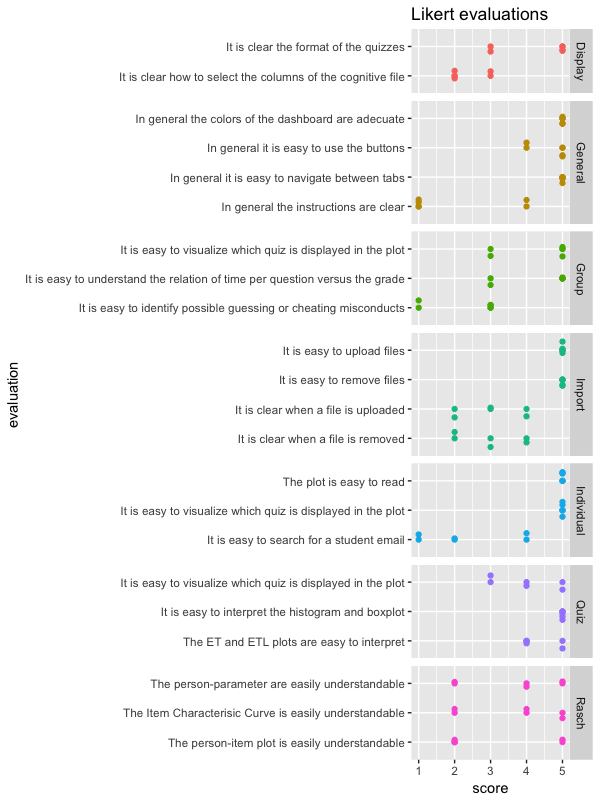
\includegraphics[width=\linewidth]{img/likert.png}
\caption{Evaluations in likert scale.}
\label{img:likert}
\end{figure}

By analysing the qualitative and the Likert evaluations, we can give more general areas of improvement. Concerning the lanalytics package, the majority of the plots were useful, but improvements regarding the titles, labels and additional characteristics were given. This is important because of shows that the content of the package is useful itself. On the other hand, for the lanalytics dashboard, the general concept and idea of the dashboard are attractive itself, also the general layout and proposed design. The area of improvement is on the instructions and analysis examples. If the instructors find difficult to use a tool that is designed to help them in their quiz analysis, then it is probable that they will not use it. For this reason, a detailed improvement on the instructions is suggested. Then, another user experience evaluations will be required.


